\chapter{نمودارهای فعالیت}
({\color{red} بهنگام‌سازی شد: افزودن نام مشخص کنشگر و خطوط شنا به طور کامل})
\\
برای هرکدام از موارد کاربرد، یک نمودار فعالیت رسم شده است که نام آن با نام مورد کاربرد رسم شده یکسان است.
\section{اضافه کردن پروژه}
\begin{figure}[H]
	\centering
	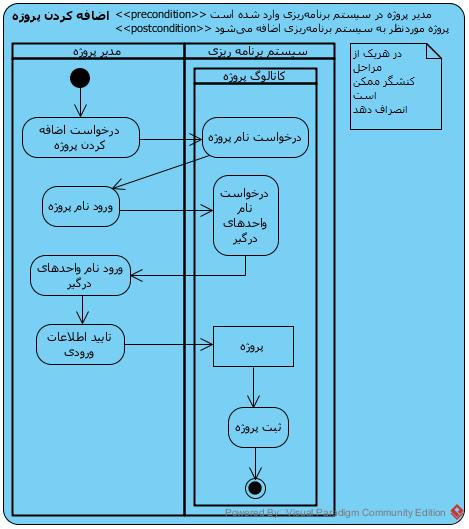
\includegraphics[scale=0.9]{img/activity/AddProjectToOrganization}
	\caption{اضافه کردن پروژه}
\end{figure}

\section{اضافه کردن سیستم به پروژه}
\begin{figure}[H]
	\centering
	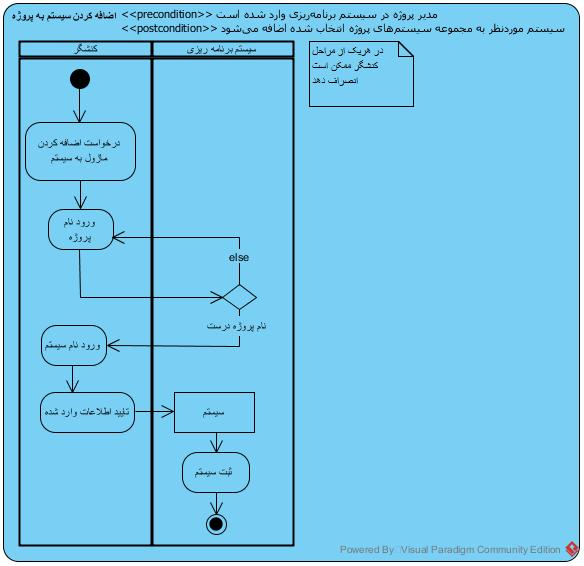
\includegraphics[scale=0.7]{img/activity/AddSystemToProject}
	\caption{اضافه کردن سیستم به پروژه}
\end{figure}

\section{اضافه کردن ماژول به سیستم}
\begin{figure}[H]
	\centering
	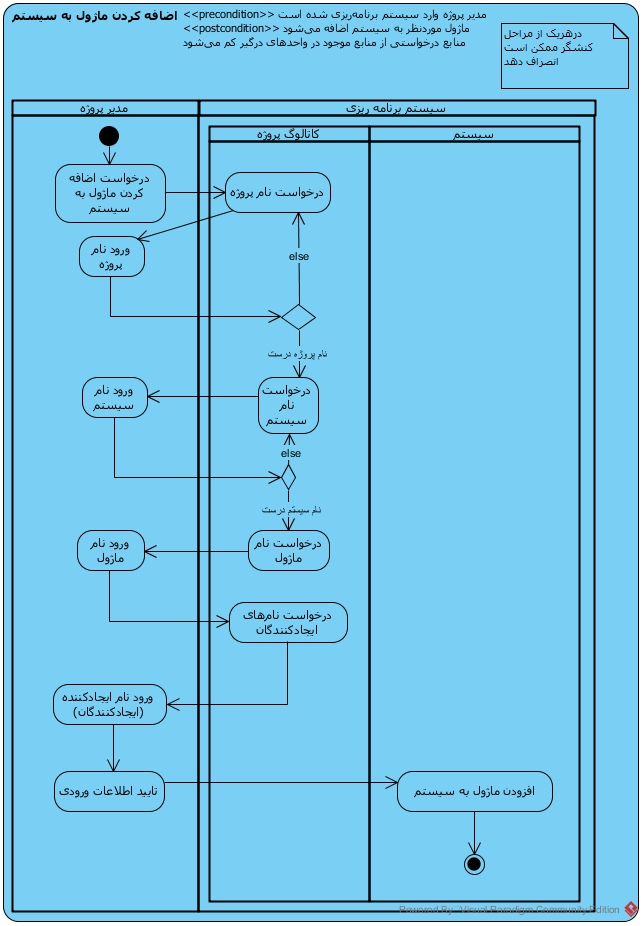
\includegraphics[scale=0.6]{img/activity/AddModuleToSystem}
	\caption{اضافه کردن ماژول به سیستم}
\end{figure}

\section{اضافه کردن منبع به واحد سازمان}
\begin{figure}[H]
	\centering
	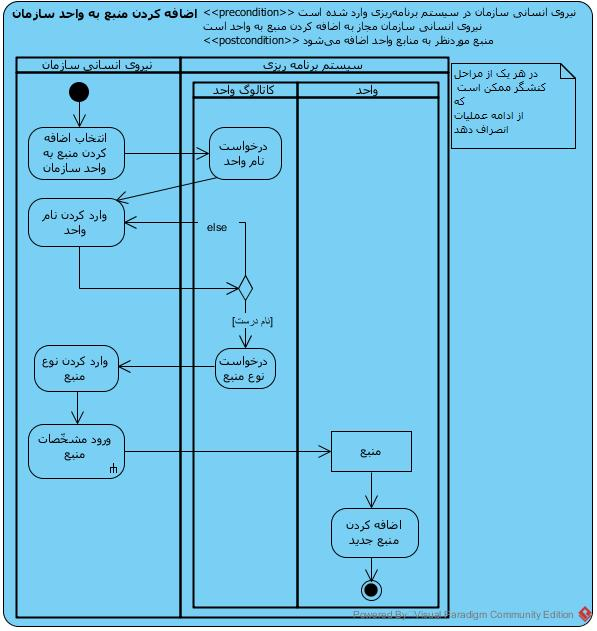
\includegraphics[scale=0.8]{img/activity/AddResourceToUnit}
	\caption{اضافه کردن منبع به واحد سازمان}
\end{figure}

\section{افزودن واحد به سازمان}
\begin{figure}[H]
	\centering
	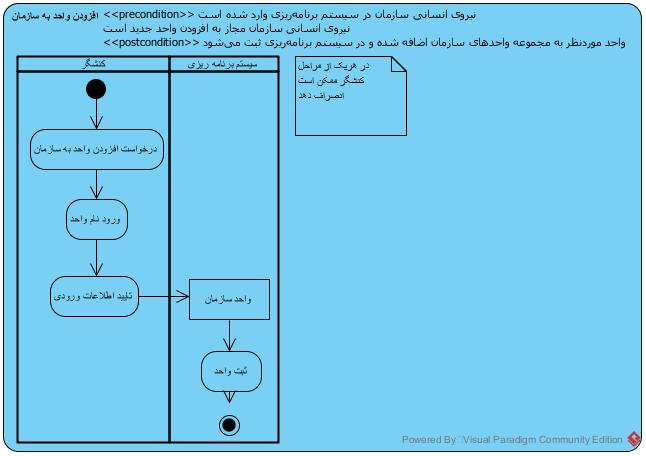
\includegraphics[scale=0.7]{img/activity/AddUnitToOrganization}
	\caption{افزودن واحد به سازمان}
\end{figure}


\section{انتخاب منبع}
\begin{figure}[H]
	\centering
	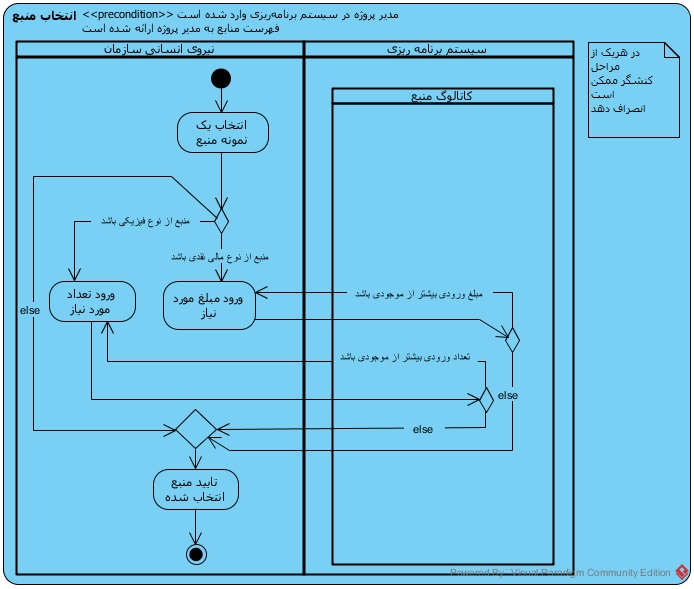
\includegraphics[scale=0.7]{img/activity/ResourceSelection}
	\caption{انتخاب منبع}
\end{figure}


\section{تخصیص منبع به پروژه}
\begin{figure}[H]
	\centering
	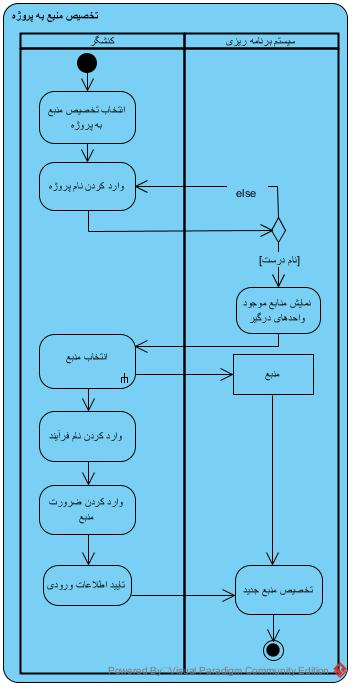
\includegraphics[scale=0.65]{img/activity/AllocateResourceToProject}
	\caption{تخصیص منبع به پروژه}
\end{figure}

\section{تعیین سطح دسترسی کاربر دیگر}
\begin{figure}[H]
	\centering
	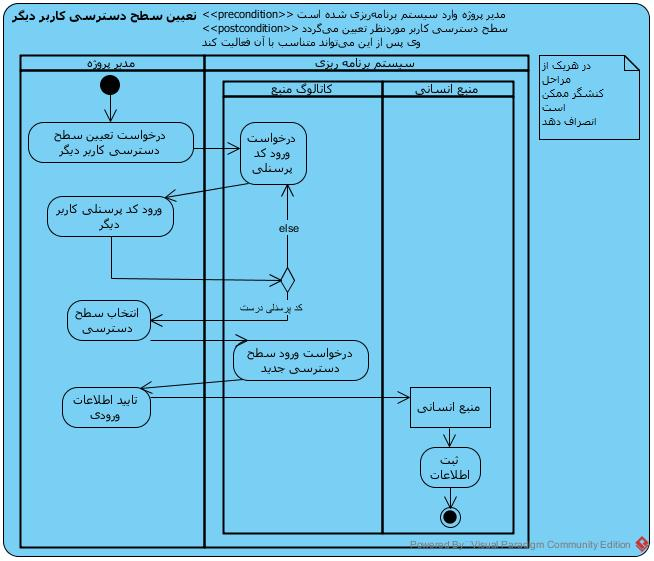
\includegraphics[scale=0.8]{img/activity/SetUserAccessLevel}
	\caption{تعیین سطح دسترسی کاربر دیگر}
\end{figure}


\section{تعیین عملیات مجاز یک سطح دسترسی}
\begin{figure}[H]
	\centering
	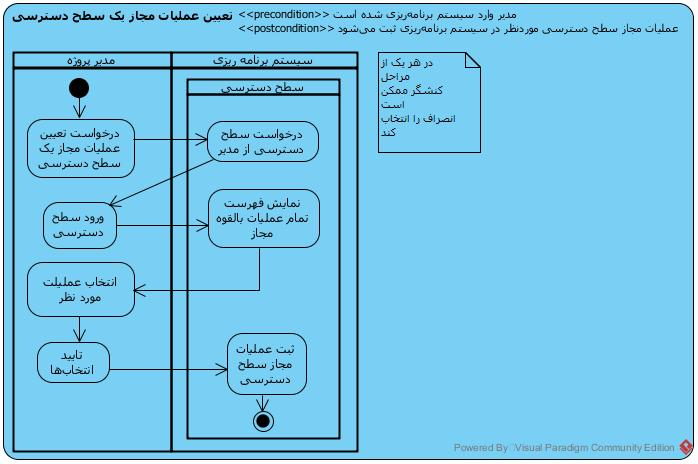
\includegraphics[scale=0.7]{img/activity/SetPermissions}
	\caption{تعیین عملیات مجاز یک سطح دسترسی}
\end{figure}


\section{تغییر سطح دسترسی کاربر دیگر}
\begin{figure}[H]
	\centering
	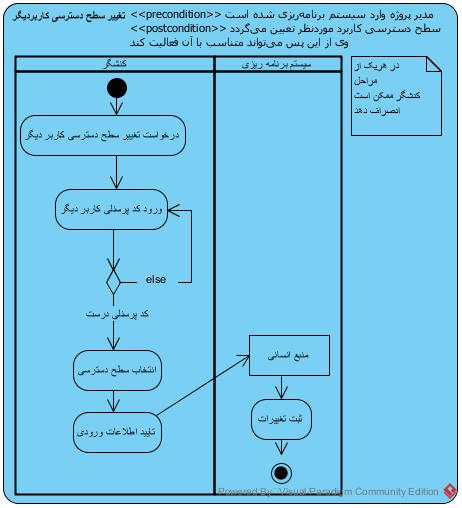
\includegraphics[scale=0.8]{img/activity/ChangeAccessLevel}
	\caption{تغییر سطح دسترسی کاربر دیگر}
\end{figure}


\section{تغییر مشخصات یک منبع}
\begin{figure}[H]
	\centering
	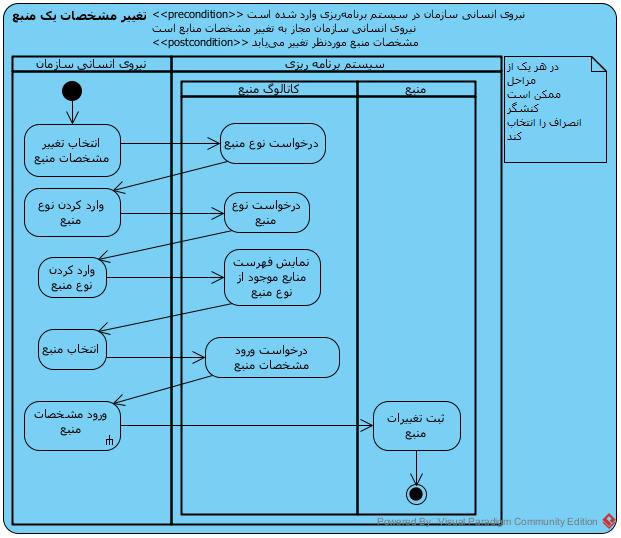
\includegraphics[scale=0.9]{img/activity/EditResourceAttributes}
	\caption{تغییر مشخصات یک منبع}
\end{figure}


\section{تهیه نسخه پشتیبان سیستم برنامه ریزی}
\begin{figure}[H]
	\centering
	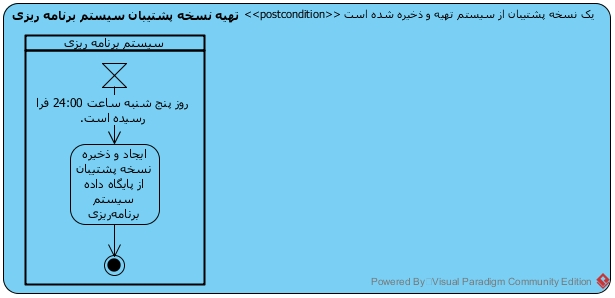
\includegraphics[scale=0.8]{img/activity/Support}
	\caption{تهیه نسخه پشتیبان سیستم برنامه ریزی}
\end{figure}

\section{ثبت تعداد استفاده‌کنندگان پروژه نرم‌افزاری}
\begin{figure}[H]
	\centering
	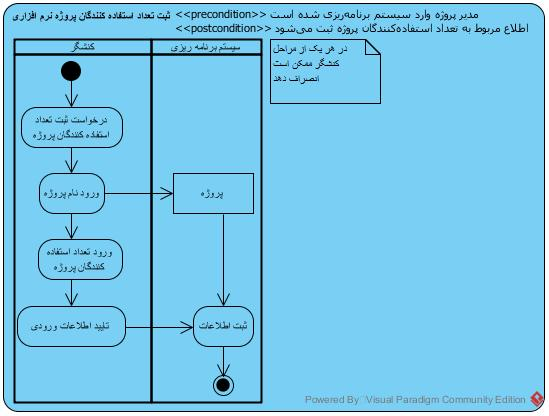
\includegraphics[scale=0.7]{img/activity/AddUsersCount}
	\caption{ثبت تعداد استفاده‌کنندگان پروژه نرم‌افزاری}
\end{figure}


\section{ثبت تغییر ماژول یک سیستم}
\begin{figure}[H]
	\centering
	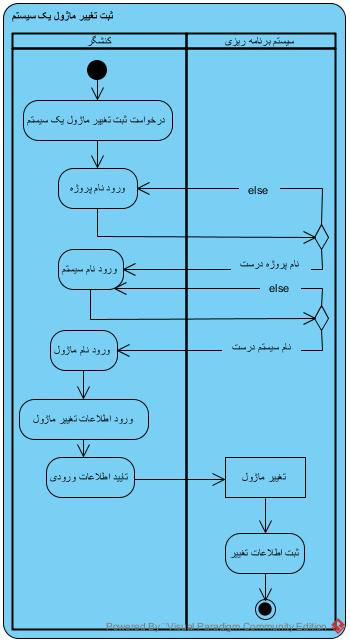
\includegraphics[scale=0.6]{img/activity/AddModuleModification}
	\caption{ثبت تغییر ماژول یک سیستم}
\end{figure}


\section{ثبت تکنولوژی مورد استفاده پروژه نرم‌افزاری}
\begin{figure}[H]
	\centering
	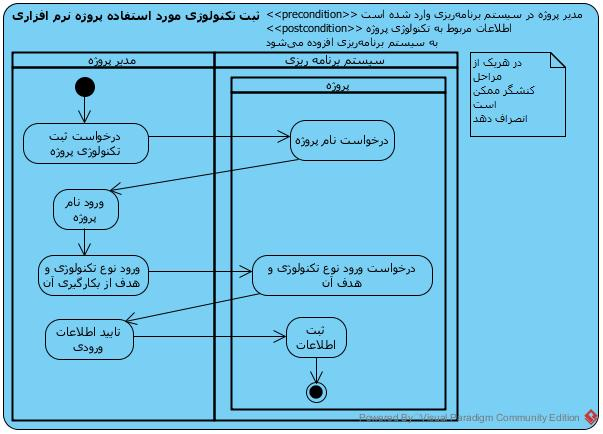
\includegraphics[scale=0.7]{img/activity/AddTechnology}
	\caption{ثبت تکنولوژی مورد استفاده پروژه نرم افزاری}
\end{figure}

\section{ثبت‌نام در سیستم برنامه‌ریزی}
\begin{figure}[H]
	\centering
	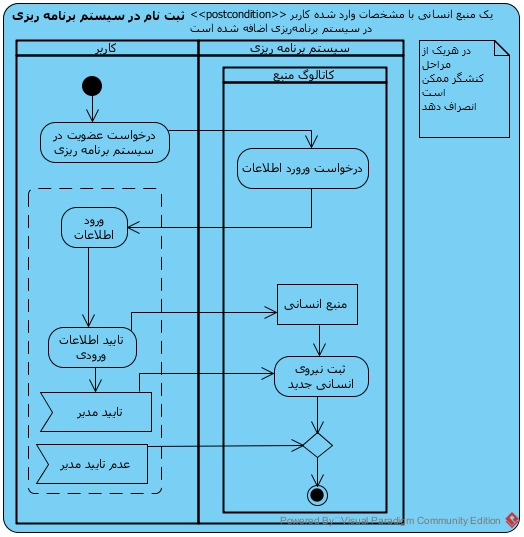
\includegraphics[scale=0.8]{img/activity/SignUp}
	\caption{ثبت نام در سیستم برنامه‌ریزی}
\end{figure}

\section{ثبت نیازمندی کنونی واحد سازمان}
\begin{figure}[H]
	\centering
	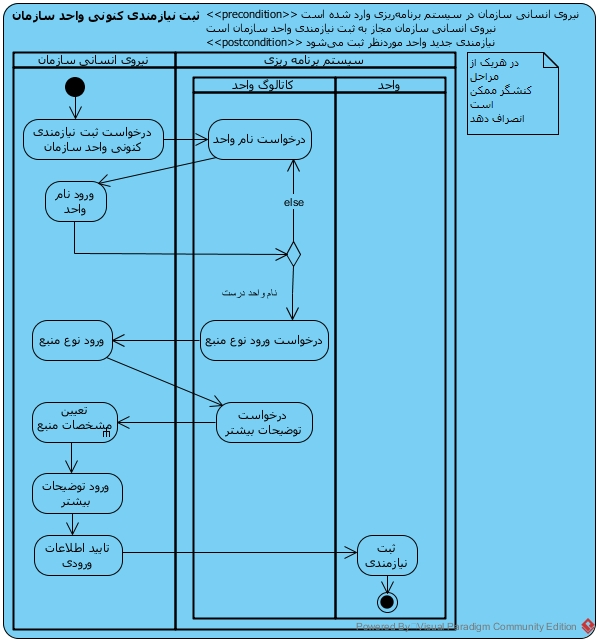
\includegraphics[scale=0.7]{img/activity/AddRequirementToUnit}
	\caption{ثبت نیازمندی کنونی واحد سازمان}
\end{figure}


\section{اضافه کردن نیازمندی به پروژه}
\begin{figure}[H]
	\centering
	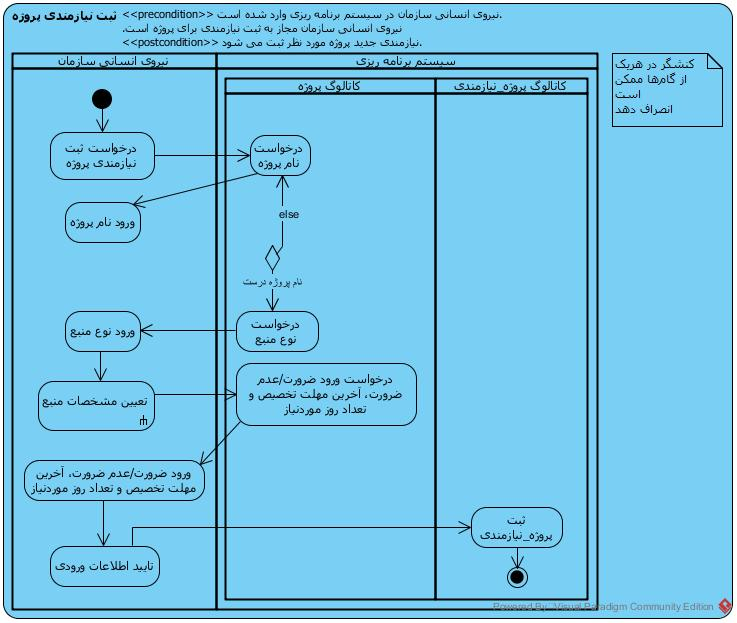
\includegraphics[scale=0.7]{img/activity/AddRequirementToProject}
	\caption{اضافه کردن نیازمندی به پروژه}
\end{figure}

\section{جستجو در پروژه‌ها برای تخمین منبع}
\begin{figure}[H]
	\centering
	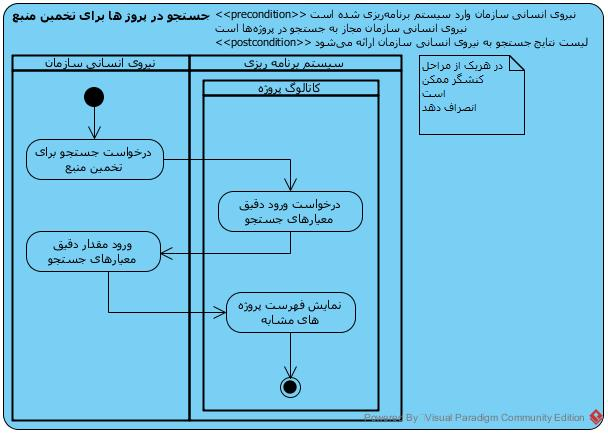
\includegraphics[scale=0.8]{img/activity/SearchInProjects}
	\caption{جستجو در پروژه‌ها برای تخمین منبع}
\end{figure}

\section{جستجو در پروژه‌ها برای یافتن نیازمندی‌های ضروری}
\begin{figure}[H]
	\centering
	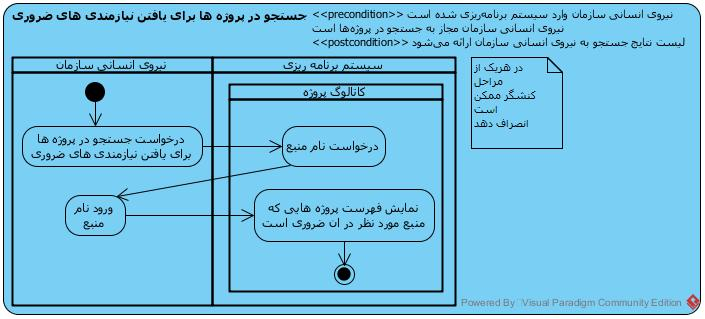
\includegraphics[scale=0.7]{img/activity/SearchForEssentialRequirements}
	\caption{جستجو در پروژه‌ها برای یافتن نیازمندی‌های ضروری}
\end{figure}


\section{خروج از سیستم}
\begin{figure}[H]
	\centering
	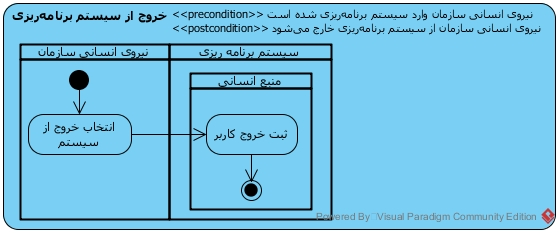
\includegraphics[scale=0.8]{img/activity/SignOut}
	\caption{خروج از سیستم}
\end{figure}


\section{دریافت گزارش جریان چرخشی مصرف منابع موجود}
\begin{figure}[H]
	\centering
	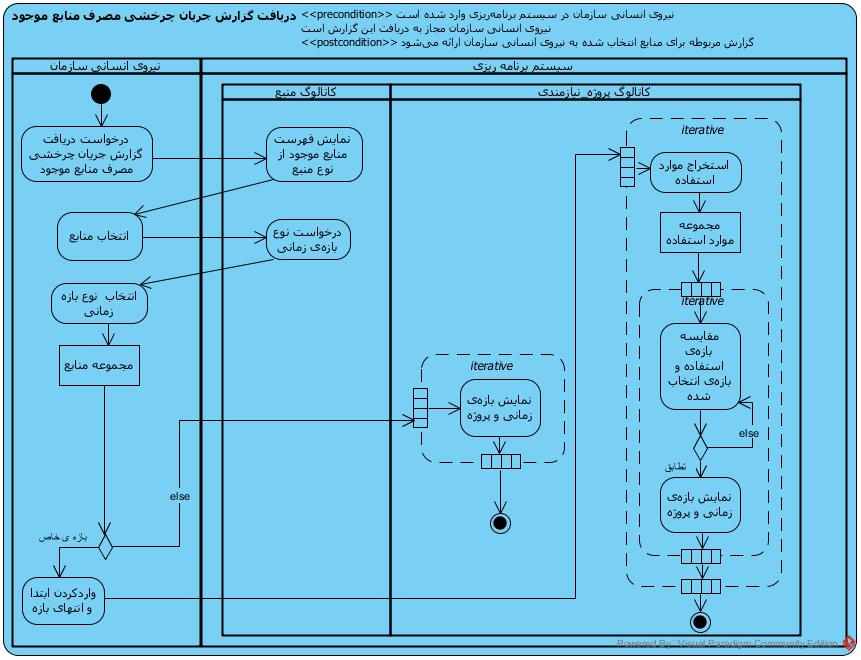
\includegraphics[scale=0.6]{img/activity/UsageFlowReport}
	\caption{دریافت گزارش جریان چرخشی مصرف منابع موجود}
\end{figure}


\newpage
\section{دریافت گزارش منابع موجود}
({\color{red} بهنگام‌سازی شد.})
\begin{figure}[H]
	\centering
	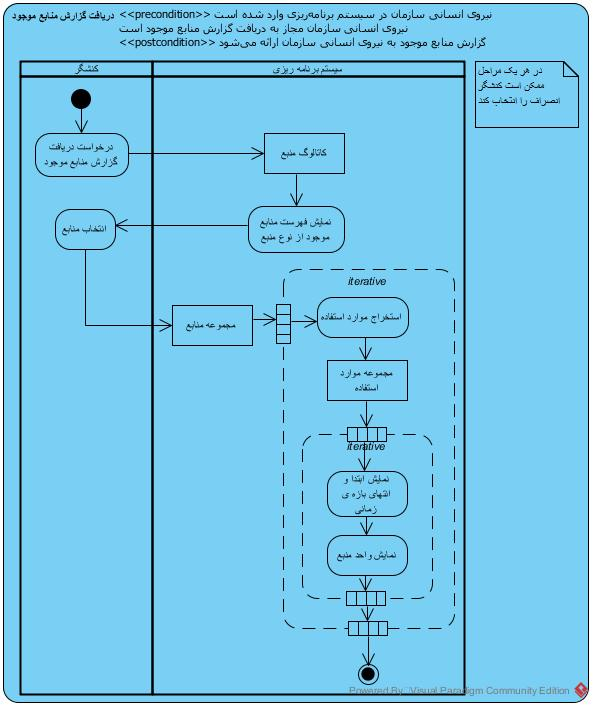
\includegraphics[scale=0.65]{img/activity/AvailableResourcesReport}
	\caption{دریافت گزارش منابع موجود}
\end{figure}


\section{دریافت گزارش منابع مورد نیاز}
\begin{figure}[H]
	\centering
	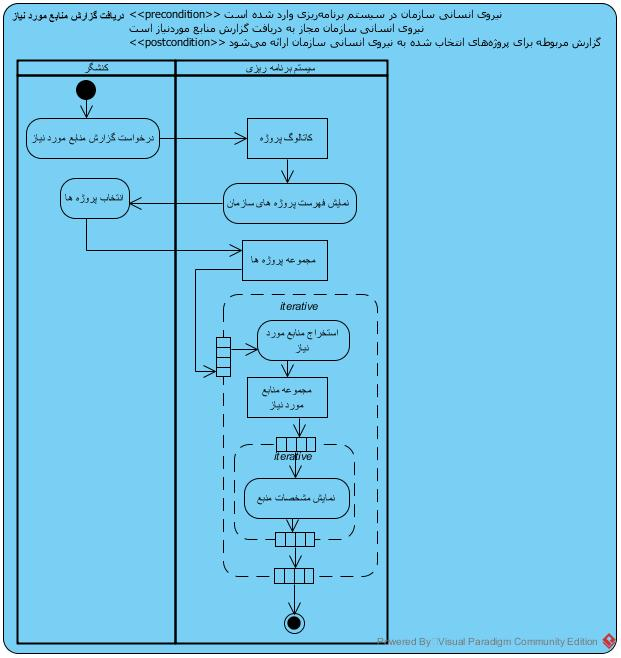
\includegraphics[scale=0.6]{img/activity/RequiredResourcesReport}
	\caption{دریافت گزارش منابع مورد نیاز}
\end{figure}

\section{مشاهده پروژه}
\begin{figure}[H]
	\centering
	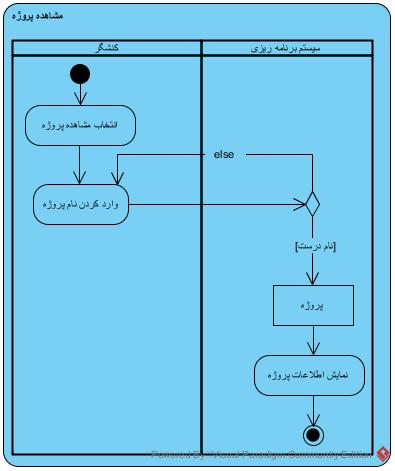
\includegraphics[scale=0.8]{img/activity/ViewProject}
	\caption{مشاهده پروژه}
\end{figure}


\section{مشاهده فهرست پروژه‌ها}
\begin{figure}[H]
	\centering
	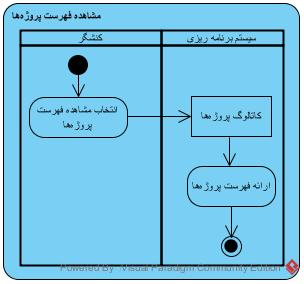
\includegraphics[scale=0.8]{img/activity/ViewListOfProjects}
	\caption{مشاهده فهرست پروژه‌ها}
\end{figure}


\section{مشاهده فهرست منابع یک واحد}
\begin{figure}[H]
	\centering
	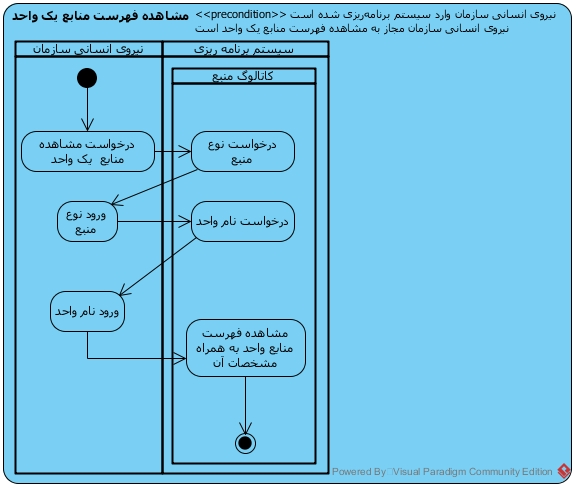
\includegraphics[scale=0.8]{img/activity/ViewListOfResources}
	\caption{مشاهده فهرست منابع یک واحد}
\end{figure}

\section{مشاهده فهرست نیازمندی‌های یک واحد}
\begin{figure}[H]
	\centering
	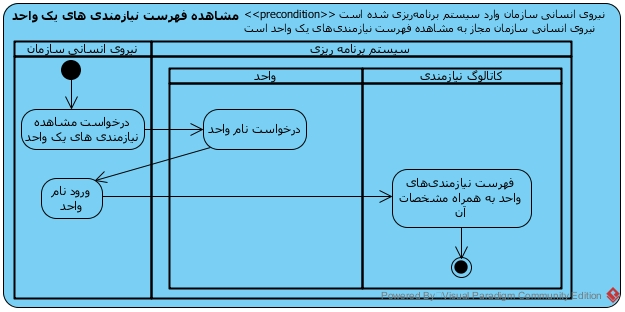
\includegraphics[scale=0.7]{img/activity/ViewListOfRequirements}
	\caption{مشاهده فهرست نیازمندی‌های یک واحد}
\end{figure}


\section{مشاهده مشخصات یک منبع}
\begin{figure}[H]
	\centering
	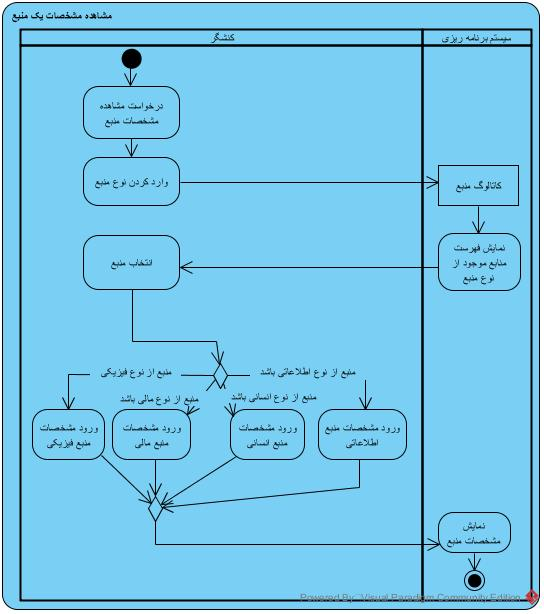
\includegraphics[scale=0.7]{img/activity/ViewResourceAttributes}
	\caption{مشاهده مشخصات یک منبع}
\end{figure}

\section{ورود به سیستم}
\begin{figure}[H]
	\centering
	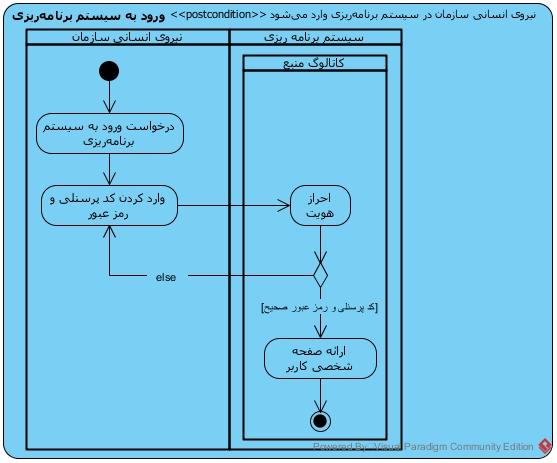
\includegraphics[scale=0.8]{img/activity/SignIn}
	\caption{ورود به سیستم}
\end{figure}


\section{ورود مشخصات منبع}
\begin{figure}[H]
	\centering
	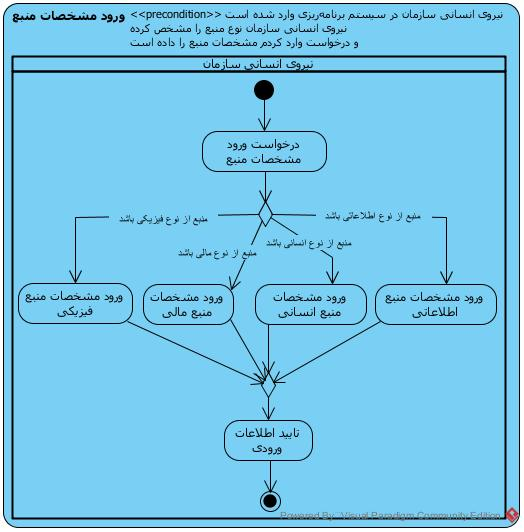
\includegraphics[scale=0.8]{img/activity/EnterResourceAttributes}
	\caption{ورود مشخصات منبع}
\end{figure}